\section{Remap}
Doordat schermen in 3 dimensies gedraaid zijn is er nood aan een correctie van het perspectief. Dit is onder meer nodig voor het lezen van de barcode en het weergeven van foto's. Het basisalgoritme die hiervoor gebruikt wordt zal bron- en bestemmingshoeken gebruiken als invoer. Deze hoeken zijn respectievelijk de start- en eindhoeken. De foto zal naar de bestemmingshoeken worden getransformeerd. Er zal per lijst van hoeken een matrix worden berekent nadat de coefficiënten berekend zijn geweest .
$$ \begin{bmatrix}
x_1 & x_2 & x_3 \\ y_1 & y_2 & y_3 \\ 1 & 1 & 1
\end{bmatrix} \begin{bmatrix}
\lambda \\ \mu \\ \tau
\end{bmatrix} =
\begin{bmatrix}
x_4 \\ y_4 \\ 1
\end{bmatrix}
$$
$$ \begin{bmatrix}
\lambda \\ \mu \\ \tau
\end{bmatrix} =\begin{bmatrix}
x_1 & x_2 & x_3 \\ y_1 & y_2 & y_3 \\ 1 & 1 & 1
\end{bmatrix}^{-1}
\begin{bmatrix}
x_4 \\ y_4 \\ 1
\end{bmatrix}
$$
Daarna wordt de 3x3 matrix geschaald met de gevonden coefficiënten.
$$
\begin{bmatrix}
\lambda x_1 & \mu x_2 & \tau x_3 \\ \lambda y_1 & \mu y_2 & \tau y_3 \\ \lambda & \mu & \tau
\end{bmatrix}
$$
De twee matrices A en B, respecitivelijk met de bron- en bestemmingshoeken, worden gebruikt om de transformatiematrix te berekenen.
$$ C = AB^{-1}$$
Deze zal elke bestemmings pixel en de bron pixel geven aan de hand van:
$$
\begin{bmatrix}
x' \\ y' \\ z'
\end{bmatrix} = C\begin{bmatrix}
x \\ y \\ 1
\end{bmatrix}
$$
$$x_{nieuw} = x'/z'$$  
$$y_{nieuw} = y'/z'$$
Een simpel algorithme zal over alle pixels (dit zijn breedte $ * $ lengte aantal pixels) gaan en de correct kleur toevoegen, zie figuur \ref{mappedfoto}. \cite{map}
\begin{figure}
\center
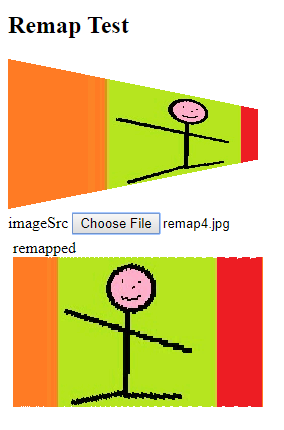
\includegraphics[scale=1]{remapEx}
\caption{Voorbeeld van een remapped foto}
\label{mappedfoto}
\end{figure}




